\section{Results}
\label{sec:results}
We applied both our methods to data from the KV450 survey and computed the ratio of observed and modeled correlation functions. Furthermore, we conducted numerical simulations investigating the same issue: A $100\,\rm{deg}^2$ field in the Scinet Light Cone Simulations (SLICS) \citep{2018MNRAS.481.1337H} was randomly separated into 10 percentiles. For each tomographic redshift bin of each percentile, galaxies were placed to trace the respective redshift distribution. Afterwards, their expected shear was determined (shape-noise in the form of intrinsic ellipticities of galaxies was not included). This was compared to a set of simulations where the galaxies were simply distributed according to the combined redshift distribution of each respective tomographic bin\todo{Catherine, is this what you did? If you are unhappy with any of these explanations, or feel like I missed something, please feel free to add it :)}. As in \citet{2018arXiv181206076H}, we have separated the data in 5 tomographic redshift bins and performed our analysis for a cross-correlation of all bins. The result can be seen in Figure \ref{fig:all_xis}.
	\begin{figure}
	\centering
	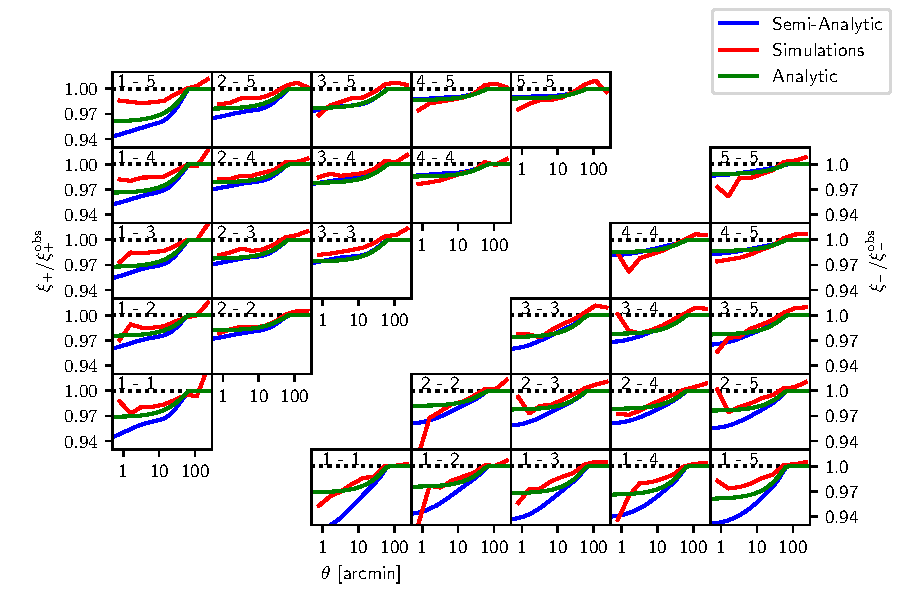
\includegraphics[width=1\textwidth]{images/allxis_0111.pdf}
	\caption{The ratio of observed to modeled correlation functions for the analytic method (green), the semi-analytic method (blue) and the numerical simulations (red) for a cross-correlation of all redshift bins.}
	\label{fig:all_xis}
	\end{figure}
We can see that for high redshift bins, the analytic and the semi-analytic methods are consistent, whereas for low redshift bins they significantly diverge. We explain this due to the facts that the analyic method uses simplifications that are redshift-dependent and only hold for small variations in redshift, which is not fulfilled in the low redshift bins.\todo{Should I include the plot number density vs average redshift from the talk? Maybe in the appendix to avoid too many Figures?}\footnote{We also observe that in the semi-analytic model, $\xi_-$ seems to be much stronger affected by this effect: Following Equation \eqref{eq:xipm-pkappa}, $\xi_+$ is computed by filtering the power spectrum with the 0-th order Bessel function. This function peaks at $\ell\theta=0$, meaning that for all values of $\theta$, the correlation function $\xi_+$ is sensitive to small values of $\ell$, corresponding to large separations $\theta$. However, $\xi_-$ is obtained by filtering with the 4-th order Bessel function, which peaks at approximately $\ell\theta\approx 5$, so for different $\theta$ this function is sensitive to varying parts of the convergence power spectrum. A more detailed analysis of this can be found in the Appendix of \citet{2017MNRAS.471.4412K}.}

The simulations seem to be in rough agreement with the models, but there are some features that can not be explained. Especially we observe that the ratios of the correlation functions for large values of $\theta$ seem to consistently surpass unity, which can not be explained by our models. The simulations seem to be in rough agreement with the models, but there are some significant differences. After a thorough analysis we explain these discrepancies the following way: The simulations were performed on a $100\,\rm{deg}^2$ field, which means that shot-noise of the fields plays a significant role. After performing the same simulations for a different distribution of depth between the pointings and obtaining completely different results, we are quite certain that this is the dominating effect. The implications of this and possible mitigation strategies will be discussed in Section \ref{sec:discussion}.


As the next step we computed a reference correlation function given a fiducial cosmology for each combination of redshift bins, and modified said correlation function according to our semi-analytic model. Then we ran a Markov-Chain Monte Carlo simulation\footnote{The code for this was developed by Jan-Luca van den Busch and used in a modified version.} to check for a potential bias in the cosmological parameters, using the covariance-matrix computed in \citet{2017MNRAS.465.1454H}. As our main interest lies in the $\Omega_{\rm m}$ - $\sigma_8$ combination, we restricted our analysis to those two parameters. As can be seen in Figure \ref{fig:mcmc_kids}, the impact of varying depth is noticeable, but insignificant compared to the uncertainties. However, to get a rough estimate for the impact on a Euclid-like survey, we divided the used covariance-matrix by 30, to account for the increased survey area. As can be seen in Figure \ref{fig:mcmc_euclid}, here the impact on both $\Omega_{\rm m}$ and $\sigma_8$ is significant, however it seems that the parameter $S_8$ is extremely robust against this effect.

To estimate the B-Modes created by this effect, we have extracted the \emph{Complete Orthogonal Sets of E- and B-Mode Integrals} (COSEBIS, compare \citet{2010A&A...520A.116S}), once of a reference set of correlation functions, to estimate numerical inaccuracies,\footnote{For a reference correlation function the B-Modes should be consistent with zero.} and then for the correlation functions that have been modified to account for a varying depth. We report a consistent B-Mode pattern across all redshift-bins, which can be seen in Figure \ref{fig:bmodes_cosebi}. Although we did not determine the error bars, that a KiDS-like survey would imply on those functions, \citet{2018arXiv181110596A} calculated the COSEBIs of the KV450 survey for the same range in $\theta$. The measured B-Modes were about one order of magnitude higher than the ones created by the varying depth, and still found to be not significant. Given these facts, we conclude that the creation of B-Modes due to varying depth in the KV450 survey is not significant. However, the pattern seems to be very characteristic, so when one encounters B-Modes in next generation surveys, which show a similar pattern, this would suggest that they are created by a similar effect (although we can not exclude other effects that just create the same B-Mode pattern). We also note that the difference in E-Modes is as large as the B-Modes, which suggests that any significant change in the cosmological parameters due to a varying depth will also yield the significant detection of B-Modes.

\begin{figure}
\centering
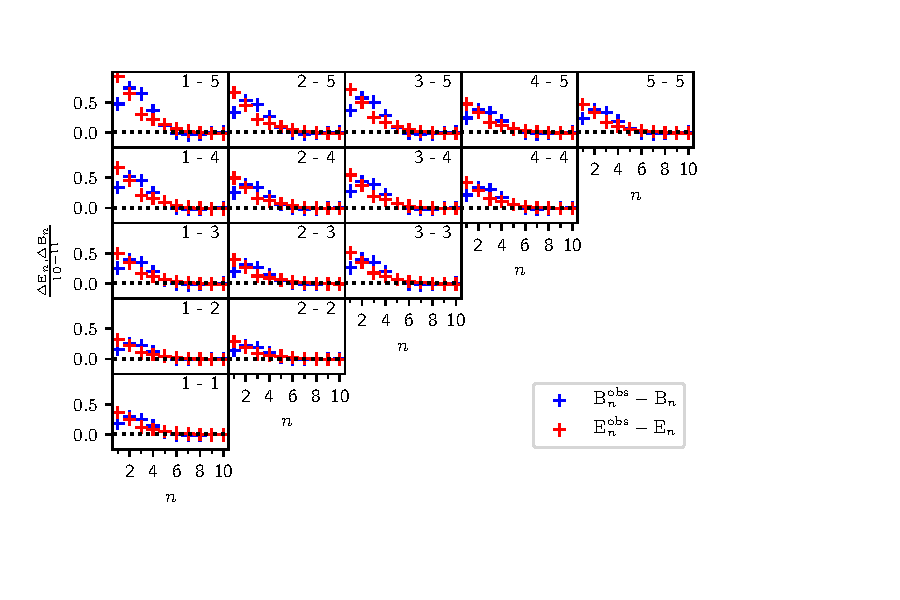
\includegraphics[width = \textwidth, trim = {0 1.5cm 2.5cm 0}, clip]{images/eandbmodes0p5t100.pdf}
\caption{Difference in the logarithmic E- and B-modes between the reference and the observed correlation functions for an angular range of $\theta_{\rm{min}}=0.\!^\prime 5,\,\theta_{\rm{max}}=100\arcmin$.}
\label{fig:bmodes_cosebi}
\end{figure}
